\documentclass[12pt]{article}
\title{Maths Question Paper}
\author{Indrajeet Shelake}
\date{16/11/2022}
\pagenumbering{roman}

\usepackage{amsmath}

\usepackage{graphicx}
\graphicspath{{./ButterflyImg.jpg}}

\usepackage{caption}
\usepackage{subcaption}

\usepackage{csvsimple}

\begin{document}
\maketitle
\newpage
\tableofcontents

\newpage
\section{Maths Paper}
\subsection*{Section I}
\textbf{Q1) Solve the following quadratic equation.\\\\}
\begin{equation*}
x^2-5x+6 = 0 
\end{equation*}
\\
\textbf{Q2) Differentiate w.r.t.x.\\\\} 
1) cos($x^2+a^2$) \\\\
2) $\sqrt{x}$ \\\\
3) $\log{(tanx)}$ \\




\subsection*{Section II}
\textbf{Q3) Find the inverse of following matrices by using adjoint method.\\\\}
1) $ A = 
\begin{bmatrix}
0 & 1 & 2 \\
1 & 2 & 3 \\
3 & 1 & 1 \\
\end{bmatrix}
$ 
\\
2) $ B = 
\begin{bmatrix}
2 & 0 & -1 \\
5 & 1 & 0 \\
0 & 1 & 3 \\
\end{bmatrix}
$
\\
\textbf{Q4) Solve the following.\\\\}
1) $ x =  
\begin{vmatrix}
7 & 11 \\
2 & 3 \\
\end{vmatrix}
$
\\
2) $ y =  
\begin{vmatrix}
45 & 90 \\
1 & 0 \\
\end{vmatrix}
$
\\
\textbf{Q5) Find domain and range of the following functions.\\\\}
1) $ g(x) = 
\frac{(x+4)}{(x-2)} \\\\
$ % Domain : R-{2} and Range : R-{1} 

2) $ h(x) = 
\sqrt[3]{(x+1)}
$ 




\subsection*{Section III}
\textbf{Q6) Verify that f and g are inverse functions of each other.\\\\}
\begin{align*}
f(x) &= (x-7)/4 \\
g(x) &= 4x+7 \\
\end{align*}
\\
\textbf{Q7) Integrate the following functions w.r.t.x.\\\\}
1) $\int x^2\, dx $ \\\\
2) $\int_{0}^{4} (x-x^2)\, dx $ \\\\
3) $\int \sin{(\log{x})} \, dx $ \\




\subsection*{Section IV}
\textbf{Q8) Given is 15 X 15 scalar matrix, write the determinent of it.\\\\}
$ A = 
\begin{bmatrix}
8 & 0 & \cdots & 0 \\
0 & 8 & \cdots & 0 \\
\vdots & \vdots & \ddots  & \vdots \\
0 & 0 & 0 & 8 \\
\end{bmatrix}
$












\newpage
\section{Images}
\huge Collection of Images \\
\begin{figure}[h]
\centering
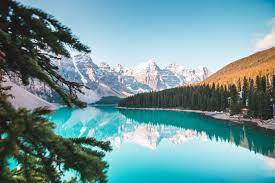
\includegraphics[scale=0.9]{./alms}
\caption{Nature}
\label{fig:Processing Mind}
\end{figure}

\begin{figure}[h]
\centering
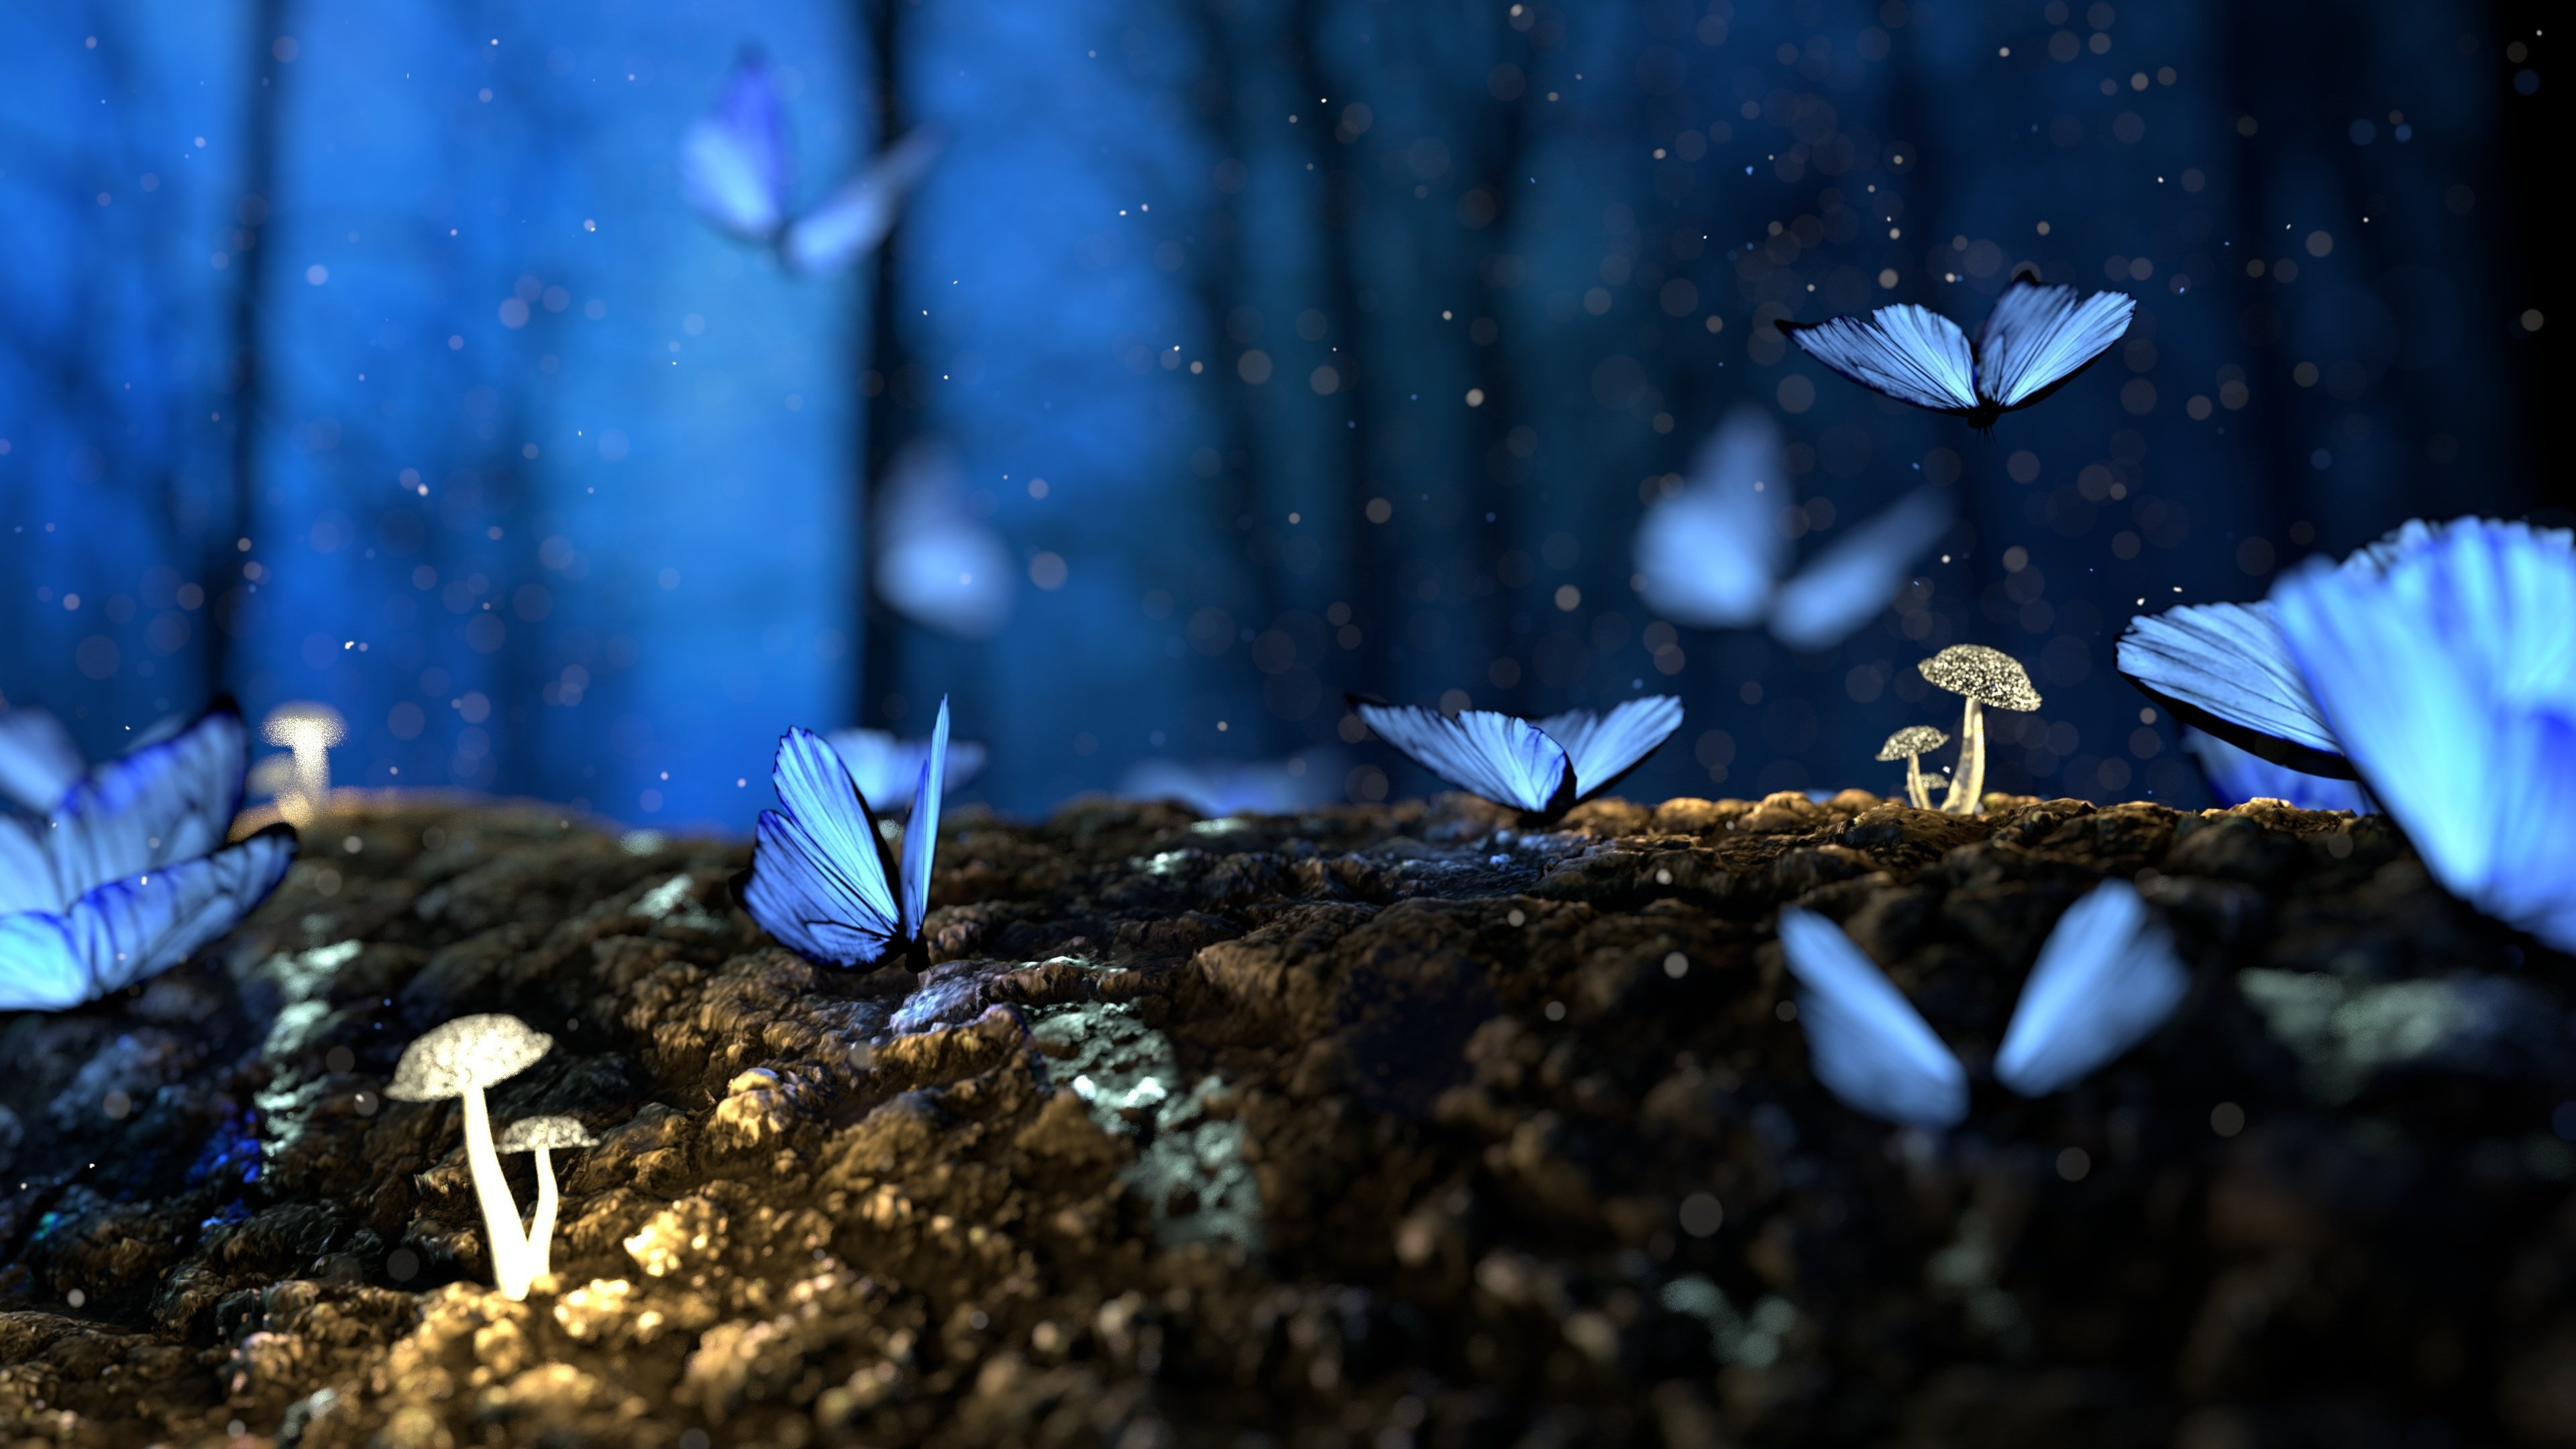
\includegraphics[scale=0.08]{ButterflyImg}
\caption{Butterfly}
\end{figure}




\newpage
\section{Table}

\begin{table}[h]
\begin{center}
\caption{Stock Market chart - current Analysis of stocks}
\label{tab:table1}

\begin{tabular}{l | l | l | l}
\hline
\textbf{Company} & \textbf{High} & \textbf{Low} & \textbf{Val.(cr.)} \\
\hline
\textbf{Infosys} & 1,588.00 & 1,562.00 & 535.74 \\ \hline
\textbf{ONGC} & 135.90 & 132.90 & 150.59 \\ \hline
\textbf{Nestle} & 19,849.30 & 19,550.05 & 93.06 \\ \hline

\end{tabular}
\end{center}
\end{table}

\newpage
\section{CSV to Latex}

\begin{table}[h]
\begin{center}
\csvautotabular{cricket.csv}
\end{center}
\end{table}

\newpage
\section{Magnet with Bibliography}

\begin{normalsize}
	Ancient people learned about magnetism from lodestones (or magnetite) which are naturally magnetized pieces of iron ore. The word magnet was adopted in Middle English from Latin magnetum "lodestone" ~\cite{1} meaning "[stone] from Magnesia",~\cite{2} a place in Anatolia where lodestones were found (today Manisa in modern-day Turkey). Lodestones, suspended so they could turn, were the first magnetic compasses. The earliest known surviving descriptions of magnets and their properties are from Anatolia, India, and China around 2500 years ago.~\cite{3}. The properties of lodestones and their affinity for iron were written of by Pliny the Elder in his encyclopedia Naturalis Historia.~\cite{4}\\	
	A straight iron magnet tends to demagnetize itself by its own magnetic field. To overcome this, the horseshoe magnet was invented by Daniel Bernoulli in 1743.~\cite{5}~\cite{6} A horseshoe magnet avoids demagnetization by returning the magnetic field lines to the opposite pole.

\begin{thebibliography} {}
\bibitem {1} Platonis Opera Archived 2018-01-14 at the Wayback Machine, Meyer and Zeller, 1839, p. 989.
\bibitem {2} The location of Magnesia is debated; it could be the region in mainland Greece or Magnesia ad Sipylum. See, for example, "Magnet". Language Hat blog. 28 May 2005. Archived from the original on 19 May 2012. Retrieved 22 March 2013.
\bibitem {3} Fowler, Michael (1997). "Historical Beginnings of Theories of Electricity and Magnetism". Archived from the original on 2008-03-15. Retrieved 2008-04-02.
\bibitem {4} Pliny the Elder, The Natural History, BOOK XXXIV. THE NATURAL HISTORY OF METALS., CHAP. 42.—THE METAL CALLED LIVE IRON Archived 2011-06-29 at the Wayback Machine. Perseus.tufts.edu. Retrieved on 2011-05-17.
\bibitem {5} Coey, J. M. D. (2009). Magnetism and magnetic materials. Cambridge: Cambridge University Press. pp. 1–3. ISBN 978-0-511-68515-6. OCLC 664016090.
\bibitem {6} "The Seven Magnetic Moments - Modern Magnets". Trinity College Dublin. Retrieved January 8, 2023.


\end{thebibliography}
\end{normalsize}


\end{document}